% !TeX root = vpl.tex

\chap{Stati: non fare sempre le stesse cose (Avanzato)}\label{ch.states}

Un programma in VPL è una lista di coppie evento-azione. Tutti gli eventi sono
controllati periodicamente e sono adottate le azioni appropriate.
Questo limita i programmi che possiamo creare; per fare cose più complesse abbiamo bisogno di un modo per specificare che alcune
coppie evento-azione sono attive in un determinato momento, mentre altre non lo sono.
Per esempio, nel \cref{ch.line}, quando il robot abbandona il nastro,
volevamo che svoltasse a sinistra o destra per cercare il nastro a seconda del lato del nastro da cui si era usciti.

La gestione degli stati è supportata nella modalità \emph{avanzata} di VPL. Clicca su
\blksm{advanced}  prima di iniziare a lavorare sui seguenti progetti.

\sect{Toc, toc}
In molti programmi, abbiamo utilizzato un pulsante per avviare il comportamento del robot e
un altro per fermarlo. Considera, però, l'interruttore di accensione sul mio computer:
%\blksm{power-button}:
Lo stesso interruttore viene usato per accendere il computer e
per spegnerlo; l'interruttore \emph{ricorda} se è in stato \bu{acceso} o in
stato \bu{spento}. L'interruttore include una piccola luce verde che indica il
suo stato attuale.

Scrivere un programma che trasforma le luci del robot quando viene urtato e
li si spegne quando urtato nuovamente.

{\raggedleft \hfill File di programma \bu{tap-on-off.aesl}}

E' utile mostrare il comportamento richiesto con un \textit{diagramma a stati}:

\begin{center}
\begin{picture}(240,45)
\thicklines
%\put(0,0){\framebox(240,40){}}
\put(20,20){\circle{40}}
\put(0,0){\makebox(40,40){\textsf{spento}}}
\put(220,20){\circle{40}}
\put(200,0){\makebox(40,40){\textsf{acceso}}}
\put(40,30){\vector(1,0){160}}
\put(0,30){\makebox(240,10){\textsf{urto $\rightarrow$ acceso}}}
\put(200,10){\vector(-1,0){160}}
\put(0,10){\makebox(240,10){\textsf{urto $\rightarrow$ spento}}}
\end{picture}
\end{center}

Nel diagramma ci sono due stati indicati da cerchi marcati con
i nomi degli stati \bu{spento} e \bu{acceso}. Dallo stato \bu{spento} il
robot può andare allo stato \bu{acceso} e tornare indietro, ma solo seguendo le
istruzioni sulle frecce. Le istruzioni descrivono quando una transizione
da uno stato all'altro può accadere e cosa succede quando si verifica:

\begin{itemize}
\item \emph{Quando} il robot è nello stato \bu{spento} \textbf{\textit{e}}
avviene l'evento \emph{urto} $\rightarrow$ \emph{accende} la luce
\textbf{\textit{e}} va nello stato \bu{acceso}.
\item \emph{Quando} il robot è nello stato \bu{acceso} \textbf{\textit{e}}
avviene l'evento \emph{urto} $\rightarrow$ \emph{spegne} la luce
\textbf{\textit{e}} va nello stato \bu{spento}.
\end{itemize}

La parola evidenziata ``\textbf{\textit{e}}'' prima della frecci~$\rightarrow$
significa che ci sono \emph{due condizioni} che devono verificarsi perchè la transizione avvenga:
 (a) Il robot deve essere in un certo stato e (b)
l'evento deve accadere. Quando entrambe le condizioni sono vere avviene la transizione, che fa eseguire sia il cambio di stato che  l'azione scritta dopo la freccia~$\rightarrow$.

E' importante comprendere che le due parti della condizione sono in dipendenti.
Nel diagramma a stati (ripetuto qui):

\begin{center}
\begin{picture}(240,45)
\thicklines
%\put(0,0){\framebox(240,40){}}
\put(20,20){\circle{40}}
\put(0,0){\makebox(40,40){\textsf{spento}}}
\put(220,20){\circle{40}}
\put(200,0){\makebox(40,40){\textsf{acceso}}}
\put(40,30){\vector(1,0){160}}
\put(0,30){\makebox(240,10){\textsf{urto $\rightarrow$ acceso}}}
\put(200,10){\vector(-1,0){160}}
\put(0,10){\makebox(240,10){\textsf{urto $\rightarrow$ spento}}}
\end{picture}
\end{center}

l'evento \emph{urto} (tap) appare due volte, ma l'azione provocata dal verificarsi dell'evento \emph{dipende} dallo stato in cui il robot si trova.

Similmente, in un singolo stato, differenti eventi possono provocare differenti azioni e transizioni a nuovi stati differenti.
nel diagramma seguente:

\begin{center}
\begin{picture}(240,80)
\thicklines
%\put(0,0){\framebox(240,80){}}
\put(30,42){\circle{30}}
\put(14,28){\makebox(30,30){\textsf{spento}}}
\put(220,22){\circle{30}}
\put(205,8){\makebox(30,30){\textsf{acceso2}}}
\put(40,57){\vector(1,0){160}}
\put(220,60){\circle{30}}
\put(205,45){\makebox(30,30){\textsf{acceso1}}}
\put(40,27){\vector(1,0){160}}
\put(0,60){\makebox(240,10){\textsf{bottone sinistro $\rightarrow$ accendi verde}}}
\put(0,30){\makebox(240,10){\textsf{bottone destro $\rightarrow$ accendi rosso}}}
\end{picture}
\end{center}

toccare il pulsante sinistro nello stato \textbf{spento} fa sì che si accenda la luce verde
e si passi nello stato \textbf{acceso1}, mentre
toccare il pulsante destro \emph{nello stesso stato} causa una diverso
azione, si accenda la luce rossa e avviene un cambiamento di uno stato diverso, verso \textbf{acceso2}.

\sect{Realizzare un diagramma a stati con le coppie evento-azione}

La \Cref{fig.turn-on-off} mostra la realizzazione del comportamento descritto dalla macchina a stati, con coppie evento-azione.


\begin{figure}
	\subfigure[Urtare per accendere e spegnere]{
		\label{fig.turn-on-off1}
		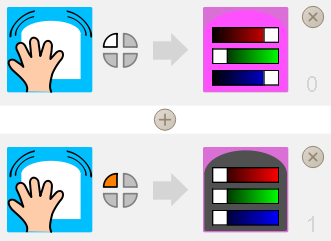
\includegraphics[width=.4\textwidth]{tap-on-off1}
	}
	\hfill
	\subfigure[Urtare per cambiare di stato]{
		\label{fig.turn-on-off2}
		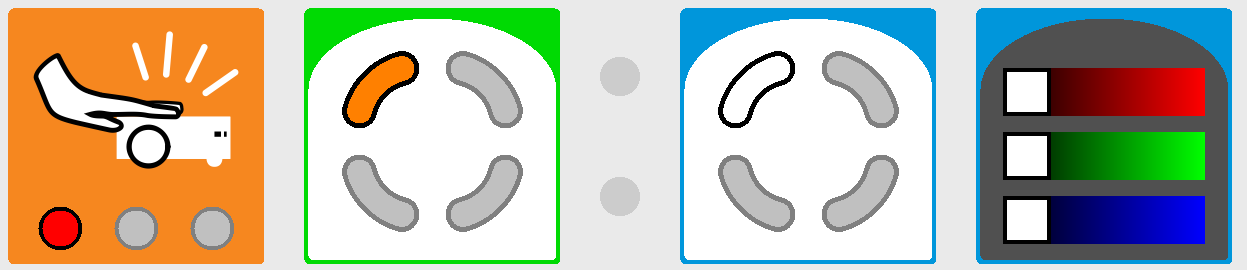
\includegraphics[width=.4\textwidth]{tap-on-off2}
	}
	\caption{L'urto ha risultati differenti in dipendenza dallo stato}
	\label{fig.turn-on-off}
\end{figure}

Nella prima coppia evento-azione, l'evento è composto dal blocco
urto con l'indicazione dello stato \blksm{tap-turn-on-state-only}: \blkc{tap-turn-on}

Uno stato è indicato da quattro quarti di un cerchio, ciascuno dei quali può essere
sia acceso (arancione) o spento (bianco). In questo programma, useremo il quarto anteriore sinistro per
indicare se la luce superiore del robot è spento o acceso. In questa coppia, questo
quarto è di colore bianco, il che significa che la luce del robot è spenta.
Pertanto, il significato della questa coppia è: se il robot è urtato e la luce è spenta, accenderla.

Analogamente, la seconda coppia evento-azione significa: se il robot
è urtato e la luce è accesa, spegnerla: \blkc{tap-turn-off}
%. Il quarto è di colore arancione, il che significa che la luce del robot è accesa

Se si guarda di nuovo il diagramma a stati, si
vedrà che solo metà del lavoro è fatto. Infatti, quando si accende o si spegne la luce, dobbiamo anche cambiare lo stato del robot da \bu{spento} a
\bu{acceso} o da \bu{acceso} a \bu{spento}. Per questo abbiamo creato due
ulteriori coppie evento-azione con il  blocco di azione \emph{stato}
\blksm{action-states}, come mostrato in \cref{fig.turn-on-off2}.

Il significato del primo è: \emph{quando}  il robot è urtato
\emph{e} lo stato è \bu{spento}, modificare lo stato di \bu{a}:
\blkc{tap-state-on}
Allo stesso modo, il significato della seconda è \emph{quando} il robot
viene urtato \emph{e} lo stato è \bu{acceso}, cambiare lo stato a \bu{spento}: \blkc{tap-state-off}

Facendo riferimento al programma completo con quattro coppie evento-azione
in \cref{fig.turn-on-off}, vediamo che
ogni evento provoca sia un'azione sulla luce che un cambiamento dello stato
del robot. Sia l'azione che il cambiamento di stato dipendono dallo stato in cui è il robot si trova, chiamato \emph{stato corrente}.

\newpage

\sect{In quanti stati può essere il robot?}

Lo stato è indicato da un cerchio diviso in quattro parti.
Quando utilizzato in un evento o in blocco l'azione dello stato, ogni quarto può essere:
\begin{itemize}
\item \textbf{Bianco}: l'elemento è \emph{spento};
\item \textbf{Arancione} : l'elemento è \emph{acceso};
\item \textbf{Grigio} : l'elemento viene ignorato.
\end{itemize}

Ad esempio, in \blksm{states}, gli elementi anteriore sinistro e posteriore destro sono accesi, l'anteriore destro è spento e quello posteriore sinistro non viene preso in considerazione,
il che significa che se \blksmpure{states} è associato a un blocco evento, l'evento si può verificare se lo stato è impostato indifferentemente su:
\begin{center}
\centering \makebox{\raisebox{-1.7em}{
\includegraphics[height=4em]{states1}}}\quad o \quad \makebox{\raisebox{-1.7em}{
\includegraphics[height=4em]{states2}}}
\end{center}

Dal momento che ciascuno dei quattro elementi può essere acceso o spento, ci sono 2 $\times$ 2 $\times$ 2 $\times$ 2  = 16 possibili stati:
\begin{quote}
\bu{(spento, spento, spento, spento), (spento, spento, spento, acceso), (spento, spento, acceso, spento), \\
\mbox{}\hspace{3em}\ldots\\
(acceso, acceso, spento, acceso), (acceso, acceso, acceso, spento), (acceso, acceso, acceso, acceso)}.
\end{quote}
La \cref{fig.all-states} enumera graficamente tutti questi stati.

\importantbox{lo stato corrente del robot viene visualizzato 
nel cerchio di LED  sulla parte superiore del robot. La \cref{fig.state-leds} mostra il robot nello stato \bu{(acceso, acceso, acceso, acceso)}.}

\trickbox[Informazione]{Quando viene eseguito un programma, lo stato iniziale è
\bu{(spento, spento, spento, spento)}:\quad \blk{state-all-off}}

\trickbox{Se non si utilizzano tutti i possibili 16 stati, ma solo 2 o 4, per esempio,
sei libero di decidere quali elementi usare per rappresentare il tuo stato.
Inoltre, se si hanno due cose diverse che si desidera codificare,
e ciascuno di essi ha due valori possibili,
è possibile utilizzare due quarti in modo indipendente.
Ecco perché la capacità di \emph{ignorare}  un quarto è molto utile!
}

\begin{figure}
	\subfigure[Tutti i possibili stati di Thymio]{
		\label{fig.all-states}
		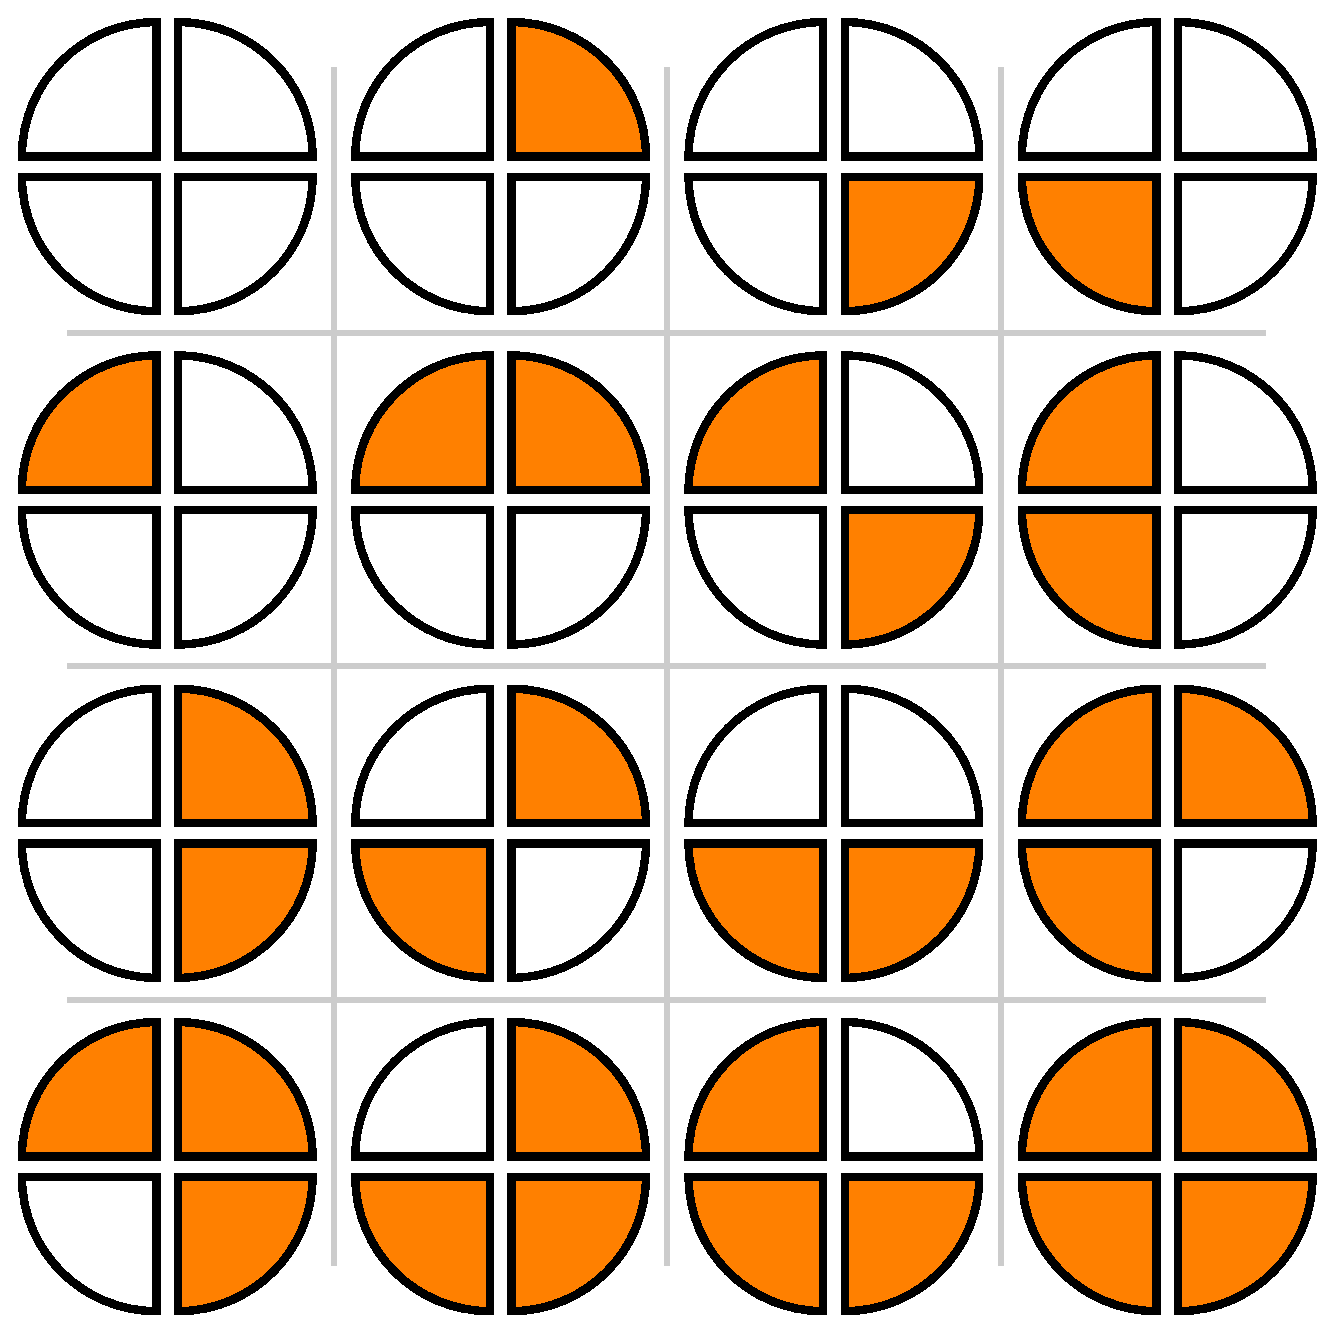
\includegraphics[width=.4\textwidth]{all-states}
	}
	\hfill
	\subfigure[Il cerchio di LED mostra lo stato]{
		\label{fig.state-leds}
		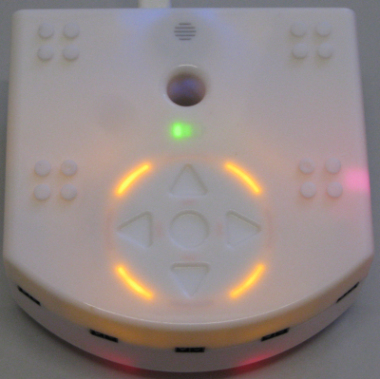
\includegraphics[width=.4\textwidth]{state-leds}
	}
	\caption{Gli stati di Thymio e la loro rappresentazione}
\end{figure}

\sect{Prendi il topo}

Scrivi un programma per implementare il comportamento di un gatto alla ricerca di un topo:
Quando si tocca il pulsante centrale, il robot gira in senso antiorario
(da destra a sinistra), alla ricerca di un topo.
Se il robot rileva un topo con il suo sensore più a destra,
gira in senso orario (da sinistra a destra) fino a quando il topo viene rilevato dal
suo sensore centrale, a quel punto si ferma (\cref{fig.cat-mouse}).

{\raggedleft \hfill File di programma \bu{mouse.aesl}}

Il seguente diagramma a stati descrive il comportamento del robot:

\begin{center}
\unitlength=1.2pt
\begin{picture}(320,35)
%\put(0,0){\framebox(320,35){}}
\put(40,10){\oval(80,20)}
\put(160,10){\oval(80,20)}
\put(280,10){\oval(80,20)}
\put(0,0){\makebox(80,20){\bu{cerca a sinistra}}}
\put(120,0){\makebox(80,20){\bu{cerca a destra}}}
\put(240,0){\makebox(80,20){\bu{trovato}}}
\put( 80,10){\vector(1,0){40}}
\put(200,10){\vector(1,0){40}}
\put(40,35){\vector(0,-1){15}}
\end{picture}
\end{center}

\begin{enumerate}
\item Quando si tocca il pulsante centrale, il robot entra nello stato
\bu{cerca a sinistra} e si sposta da destra a sinistra.
\item Quando il robot è in stato \bu{cerca a sinistra}
e rileva il topo nel sensore più a destra,
si sposta nello stato \bu{cerca a destra} e si sposta da sinistra a destra.
\item Quando il robot è nello stato \bu{cerca a destra} 
e rileva il topo con il sensore centrale,
va nello stato \bu{trovato} e si ferma.
\end{enumerate}

Il punto importante da notare è che quando il topo viene rilevato dal
sensore di centro, il robot si ferma \emph{solo} se è nello stato
\bu{cerca a destra}.
Altrimenti (se il topo viene rilevato dal sensore centrale quando il robot
è in stato \bu{cerca a sinistra}), non accade nulla.

\begin{figure}
	\subfigure[Il gatto ha trovato il topo]{\label{fig.cat-mouse}
	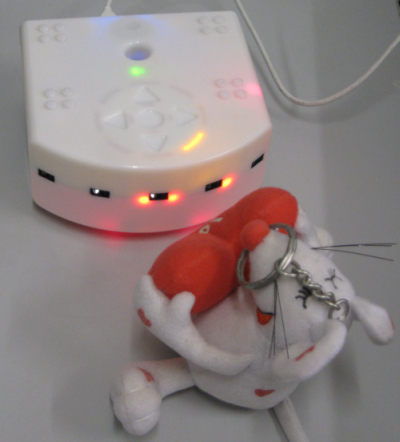
\includegraphics[width=0.4\textwidth]{cat-mouse}}
	\hfill
	\subfigure[Cerca con il sensore più a destra]{\label{fig.mouse2}
	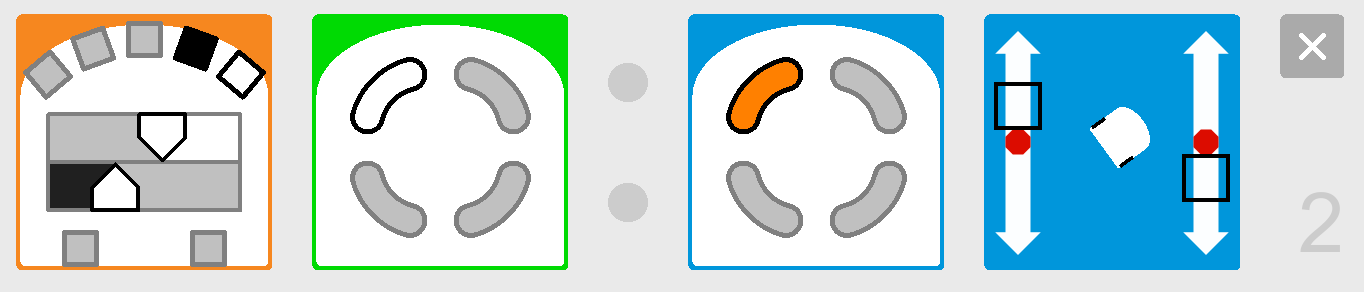
\includegraphics[width=0.4\textwidth]{mouse2}}
	\caption{Il gatto robot cerca il topo}
\end{figure}

Vediamo ora come implementare questo comportamento. Rappresentiamo lo stato del robot
con l'elemento in alto a sinistra dell'indicatore di stato.
Abbiamo scelto bianco per lo stato
\bu{cerca a sinistra} e arancione per lo stato \bu{cerca a destra}.
Poiché il programma termina quando viene rilevato il topo in stato
\bu{cerca a destra} non abbiamo bisogno di rappresentare esplicitamente lo stato \bu{trovato}.
Inizialmente, tutti gli elementi dello stato sono \bu{spenti} (bianchi).

La seguente coppia evento-azione implementa il comportamento del punto 1:
\blkc{mouse1}

Le coppie evento-azione che implementano il punto 2 sono mostrate in \cref{fig.mouse2}.
Entrambe utilizzano lo stesso evento, ma le azioni sono diverse. La prima modifica
la direzione del movimento del robot e la seconda cambia il suo stato
da \bu{cerca a sinistra} a \bu{cerca a destra}.

Il piccolo quadrato accanto al sensore più a destra è impostato su bianco in modo che l'evento
si verifichi solo quando solamente il sensore più a destra rileva il topo.

Il punto 3 è implementato dalla seguente coppia evento-azione:
\blkc{mouse3}
che fa sì che il robot si fermi quando il topo si trova direttamente davanti al sensore centrale.
Come previsto dal punto 3 questo avverrà solo durante la ricerca sulla destra: quando il robot è in stato \bu{cerca a destra} come indicato dall'elemento in arancione.

\trickbox{
Dovrete fare degli esperimeni con la distanza del topo dal robot.
Se è troppo vicino al robot, i sensori su entrambi i lati
del sensore centrale rilevano anche loro il mouse, mentre l'evento richiede
che essi \emph{non} lo rilevino.}
\vfill
\exercisebox{\thechapter.1}{
Scrivere un programma che fa danzare il robot: si gira a sinistra sul
posto per due secondi e poi si gira a destra sul posto per tre secondi.
Questi movimenti vengono ripetuti all'infinito.
}
\exercisebox{\thechapter.2(Difficile)}{
Modificare il programma per seguire una linea del \cref{ch.line} in modo che il
robot giri a sinistra quando lascia il lato destro della linea e
gira a destra quando lascia il lato sinistro della linea.
}
